\chapter{La reproducción sexual}\label{ch:g8:sexual-reproduction}

El canto de las ranas en mayo, las \omterm{def:g3:flowers-fruits-seeds:parts}{flores} del cerezo en abril, la
berrea del ciervo en otoño, un girasol que gira su cara abarrotada
hacia las abejas: en todo el mundo vivo se gasta una \omterm{prop:g3:balanced-diet:jobs}{energía} enorme en
un solo proyecto --- la generación siguiente. Los cursos anteriores
reunieron las piezas (\cref{ch:g4:animal-reproduction},
\cref{ch:g5:flower-to-fruit}); este curso las monta en una sola teoría
y hace la pregunta más afilada: ¿por qué \emph{dos} progenitores?

\begin{omfigure}
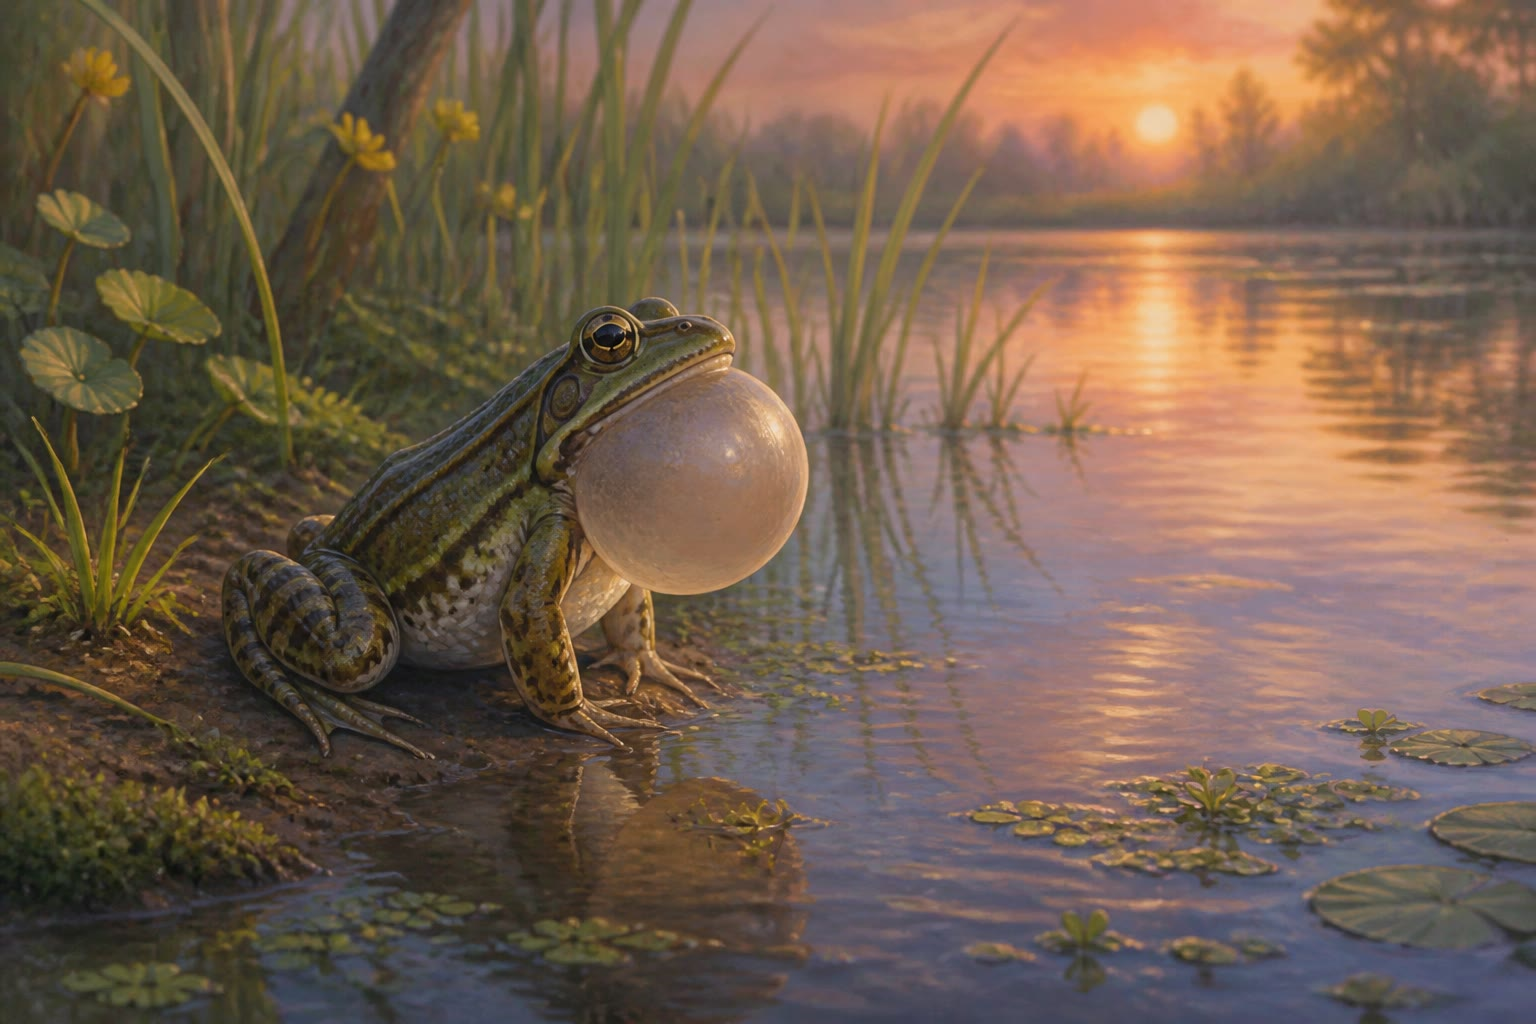
\includegraphics[width=0.6\linewidth]{images/book1/ai/g8-frog-chorus.jpg}

{\small Una \omterm{prop:g3:balanced-diet:jobs}{energía} enorme para un solo proyecto: el saco vocal
hinchado del \omterm{def:g4:animal-reproduction:sexual}{macho}, convocando a la charca al encuentro de los \omterm{def:g8:sexual-reproduction:gametes}{gametos}.}
\end{omfigure}

\section{Un mismo mecanismo en todo el mundo vivo}

\begin{definition}[Gametos]\label{def:g8:sexual-reproduction:gametes}
Las \omterm{def:g5:first-look-at-cells:cell}{células} reproductoras de la
\cref{def:g4:animal-reproduction:sexual} tienen un nombre general:
\emph{gametos}\index{gameto}. El gameto \omterm{def:g4:animal-reproduction:sexual}{masculino} (el \omterm{def:g4:animal-reproduction:sexual}{espermatozoide} en
los \omterm{def:g1:animals-around-us:animal}{animales}, la \omterm{def:g5:first-look-at-cells:cell}{célula} del grano de \omterm{def:g3:flowers-fruits-seeds:parts}{polen} en las \omterm{def:g1:plants-around-us:plant}{plantas} con \omterm{def:g3:flowers-fruits-seeds:parts}{flores}) y
el gameto \omterm{def:g4:animal-reproduction:sexual}{femenino} (la \omterm{def:g5:first-look-at-cells:cell}{célula} \omterm{def:g4:animal-reproduction:sexual}{femenina}, en un ovario o en un \omterm{def:g4:animal-reproduction:sexual}{óvulo}).
Los gametos son \omterm{def:g5:first-look-at-cells:cell}{células} sueltas (\cref{ch:g5:first-look-at-cells}), y
cada uno es medio comienzo: solo, un gameto se muere; unidos, dos hacen
una vida.
\end{definition}

\begin{proposition}[El núcleo invariable]\label{prop:g8:sexual-reproduction:core}
Allí donde hay \omterm{def:g4:animal-reproduction:sexual}{reproducción sexual} --- \omterm{prop:g3:sorting-living-things:groups}{pez} o abeto, caracol o persona
--- el \omterm{def:g6:cell-unit-of-life:parts}{núcleo} es invariable:
\begin{enumerate}
  \item dos progenitores producen \omterm{def:g8:sexual-reproduction:gametes}{gametos}, \omterm{def:g4:animal-reproduction:sexual}{masculinos} y \omterm{def:g4:animal-reproduction:sexual}{femeninos};
  \item la \emph{\omterm{def:g5:flower-to-fruit:steps}{fecundación}}: un \omterm{def:g8:sexual-reproduction:gametes}{gameto} \omterm{def:g4:animal-reproduction:sexual}{masculino} se une a un \omterm{def:g8:sexual-reproduction:gametes}{gameto}
        \omterm{def:g4:animal-reproduction:sexual}{femenino} y forma una sola \omterm{def:g5:first-look-at-cells:cell}{célula} nueva --- la \emph{\omterm{def:g5:first-look-at-cells:cell}{célula}
        \omterm{def:g4:animal-reproduction:sexual}{femenina} fecundada}, o \emph{cigoto}\index{cigoto};
  \item el \omterm{prop:g8:sexual-reproduction:core}{cigoto} se divide y se divide
        (\cref{prop:g5:first-look-at-cells:growth}) y construye un
        individuo nuevo que lleva algo de \emph{los dos} progenitores
        (\cref{rem:g4:animal-reproduction:mix}).
\end{enumerate}
Alrededor de este \omterm{def:g6:cell-unit-of-life:parts}{núcleo}, todo lo demás es variación: dónde se
encuentran los \omterm{def:g8:sexual-reproduction:gametes}{gametos}, cuántos son y quién cuida a las crías.
\end{proposition}
\admitted

\begin{example}[Las variaciones, clasificadas]\label{ex:g8:sexual-reproduction:variations}
La vieja colección se archiva sin problemas bajo el \omterm{def:g6:cell-unit-of-life:parts}{núcleo}. \omterm{def:g5:flower-to-fruit:steps}{Fecundación}
externa frente a interna
(\cref{prop:g4:animal-reproduction:where}): el sitio del encuentro.
\omterm{def:g4:animal-reproduction:ovivivi}{Ovíparo} frente a \omterm{def:g4:animal-reproduction:ovivivi}{vivíparo}
(\cref{def:g4:animal-reproduction:ovivivi}): el alojamiento del \omterm{prop:g8:sexual-reproduction:core}{cigoto}.
Los millones del bacalao frente a la cría única de la elefanta
(\cref{prop:g4:animal-reproduction:strategies}): la contabilidad de los
números. \omterm{def:g5:flower-to-fruit:steps}{Polinización} por abeja o por viento
(\cref{def:g5:flower-to-fruit:steps}): el servicio de viajes del \omterm{def:g8:sexual-reproduction:gametes}{gameto}
\omterm{def:g4:animal-reproduction:sexual}{masculino}. Un mecanismo, un catálogo de ajustes.
\end{example}

\begin{remark}[Las plantas hacen el mismo núcleo]\label{rem:g8:sexual-reproduction:plants}
Pon el \cref{ch:g5:flower-to-fruit} al lado del
\cref{ch:g4:animal-reproduction} y la correspondencia es exacta: los
\omterm{def:g3:flowers-fruits-seeds:parts}{estambres} y el \omterm{def:g3:flowers-fruits-seeds:parts}{pistilo} producen los \omterm{def:g8:sexual-reproduction:gametes}{gametos}, el tubo polínico es el
pasillo de la \omterm{def:g5:flower-to-fruit:steps}{fecundación} interna y la \omterm{def:g2:from-seed-to-plant:seed}{semilla} aloja al \omterm{def:g5:human-reproduction:pregnancy}{embrión} de la
\omterm{def:g1:plants-around-us:plant}{planta} con su fiambrera (\cref{def:g2:from-seed-to-plant:seed}). Solo
la \omterm{def:g4:plants-without-seeds:vegetative}{reproducción vegetativa}
(\cref{def:g4:plants-without-seeds:vegetative}) queda aparte --- un
progenitor, ningún \omterm{def:g8:sexual-reproduction:gametes}{gameto}, copias exactas: el contraste que afila la
pregunta de la sección siguiente.
\end{remark}

\section{¿Por qué dos progenitores?}

\begin{proposition}[La reproducción sexual baraja]\label{prop:g8:sexual-reproduction:shuffle}
Las copias de fresa de los \omterm{ex:g4:plants-without-seeds:runner}{estolones}
(\cref{rem:g4:plants-without-seeds:copy}) enseñan lo que da un solo
progenitor: igualdad. Dos progenitores dan lo contrario. Como todos los
\omterm{prop:g8:sexual-reproduction:core}{cigotos} combinan un \omterm{def:g8:sexual-reproduction:gametes}{gameto} de cada progenitor --- y, como enseñará un
capítulo posterior, ni siquiera dos \omterm{def:g8:sexual-reproduction:gametes}{gametos} de un mismo progenitor
llevan exactamente la misma herencia ---, la \omterm{def:g4:animal-reproduction:sexual}{reproducción sexual} le
reparte a cada descendiente una \emph{combinación nueva}. Los hermanos
se diferencian; no hay dos \omterm{prop:g2:from-seed-to-plant:cycle}{plántulas} iguales de una misma vaina; y la
variedad que hay dentro de cada \omterm{def:g5:biodiversity:species}{especie}
(\cref{rem:g5:biodiversity:scales}) es en buena parte obra de este
barajado.
\end{proposition}
\admitted

\begin{example}[Las dos apuestas del huerto]\label{ex:g8:sexual-reproduction:bets}
El huerto de frutales de la \cref{rem:g4:plants-without-seeds:copy}
juega a los dos juegos a sabiendas. Injertos y \omterm{met:g4:plants-without-seeds:cutting}{esquejes}: un progenitor,
copias exactas del árbol excelente --- y una sola debilidad compartida,
así que una plaga que tumbe a uno los puede tumbar a todos. Pepitas:
dos progenitores, cada \omterm{prop:g2:from-seed-to-plant:cycle}{plántula} una combinación nueva --- casi todas
del montón, algunas peores, alguna rara vez mejor que sus dos
progenitores, y ninguna igual a otra para que la barra una plaga.
Copiar ingresa el presente; barajar explora el futuro.
\end{example}

\begin{remark}[La variedad es la reserva de la especie]\label{rem:g8:sexual-reproduction:reserve}
Por qué importa el barajado más allá del huerto: la
\cref{prop:g5:biodiversity:web} enseñó redes absorbiendo golpes gracias
a la variedad de \omterm{def:g5:biodiversity:species}{especies}; dentro de una \omterm{def:g5:biodiversity:species}{especie}, la variedad de
individuos hace ese mismo papel. Cuando las \omterm{def:g6:exploring-our-environment:conditions}{condiciones} cambian --- una
enfermedad nueva, un invierno más duro --- una \omterm{def:g5:biodiversity:species}{especie} variada tiene
más probabilidades de contar con alguien que encaje en las \omterm{def:g6:exploring-our-environment:conditions}{condiciones}
nuevas. Lo que eso insinúa sobre la historia de la vida lo hará
explícito el \cref{ch:g9:how-species-change}; quédate aquí solo con que
es la \omterm{def:g4:animal-reproduction:sexual}{reproducción sexual} la que mantiene surtida esa reserva.
\end{remark}

\section{Leer la reproducción de cualquier especie}

\begin{method}[El expediente de reproducción]\label{met:g8:sexual-reproduction:dossier}
Para cualquier \omterm{def:g5:biodiversity:species}{especie}, recopila:
\begin{enumerate}
  \item \omterm{def:g8:sexual-reproduction:gametes}{gametos}: quién produce cuál y dónde;
  \item encuentro: \omterm{def:g5:flower-to-fruit:steps}{fecundación} externa o interna, y el servicio de
        viajes (agua, \omterm{prop:g4:animal-reproduction:where}{apareamiento}, polinizador, viento);
  \item alojamiento: \omterm{def:g2:animals-grow-up:born}{huevos} puestos o crías llevadas dentro; y con qué
        provisiones;
  \item números y cuidados: la posición en la línea de estrategias
        (\cref{prop:g4:animal-reproduction:strategies});
  \item estación: cuándo, y marcada por qué --- la pregunta del
        capítulo siguiente.
\end{enumerate}
\end{method}

\begin{example}[Dos expedientes uno al lado del otro]\label{ex:g8:sexual-reproduction:dossiers}
El espinoso (\cref{exo:g4:animal-reproduction:10}): \omterm{def:g8:sexual-reproduction:gametes}{gametos} soltados en
el agua, \omterm{def:g5:flower-to-fruit:steps}{fecundación} externa, \omterm{def:g2:animals-grow-up:born}{huevos} en un nido construido, decenas,
vigilados por el padre, primavera. El cerezo: \omterm{def:g8:sexual-reproduction:gametes}{gametos} en la \omterm{def:g3:flowers-fruits-seeds:parts}{flor},
\omterm{def:g5:flower-to-fruit:steps}{fecundación} interna bajando por el tubo polínico, embriones alojados en
\omterm{prop:g3:flowers-fruits-seeds:transform}{semillas} dentro de un \omterm{prop:g3:flowers-fruits-seeds:transform}{fruto}, miles, provistos y después abandonados al
servicio de reparto de los pájaros
(\cref{exo:g6:how-plants-spread:12}), con la fecha en abril. El mismo
formulario, para cualquier \omterm{def:g5:biodiversity:species}{especie}: el expediente es la teoría en uso.
\end{example}

\section{Ejercicios}

\begin{exercise}[$\star$]\label{exo:g8:sexual-reproduction:1}
Define \omterm{def:g8:sexual-reproduction:gametes}{gameto} y \omterm{prop:g8:sexual-reproduction:core}{cigoto}, y nombra los dos \omterm{def:g8:sexual-reproduction:gametes}{gametos} de los \omterm{def:g1:animals-around-us:animal}{animales} y los
de las \omterm{def:g1:plants-around-us:plant}{plantas} con \omterm{def:g3:flowers-fruits-seeds:parts}{flores}.
\end{exercise}

\begin{exercise}[$\star$]\label{exo:g8:sexual-reproduction:2}
Enuncia el \omterm{def:g6:cell-unit-of-life:parts}{núcleo} invariable en tres pasos.
\end{exercise}

\begin{exercise}[$\star$]\label{exo:g8:sexual-reproduction:3}
Archiva bajo el \omterm{def:g6:cell-unit-of-life:parts}{núcleo}: \omterm{def:g5:flower-to-fruit:steps}{fecundación} externa o interna, \omterm{def:g4:animal-reproduction:ovivivi}{ovíparo} o
\omterm{def:g4:animal-reproduction:ovivivi}{vivíparo}, millones o cría única --- ¿qué hace variar cada pareja?
\end{exercise}

\begin{exercise}[$\star$]\label{exo:g8:sexual-reproduction:4}
Empareja las partes de la \omterm{def:g1:plants-around-us:plant}{planta} con los papeles \omterm{def:g1:animals-around-us:animal}{animales}: \omterm{def:g3:flowers-fruits-seeds:parts}{estambre},
\omterm{def:g3:flowers-fruits-seeds:parts}{pistilo}, tubo polínico, \omterm{def:g2:from-seed-to-plant:seed}{semilla}.
\end{exercise}

\begin{exercise}[$\star$]\label{exo:g8:sexual-reproduction:5}
¿Qué da la reproducción de un solo progenitor que no da nunca la de
dos --- y al revés?
\end{exercise}

\begin{exercise}[$\star$]\label{exo:g8:sexual-reproduction:6}
¿Por qué se diferencian los hermanos, según la
\cref{prop:g8:sexual-reproduction:shuffle}?
\end{exercise}

\begin{exercise}[$\star\star$]\label{exo:g8:sexual-reproduction:7}
Explica las dos apuestas del huerto y cuándo es cada una la acertada.
\end{exercise}

\begin{exercise}[$\star\star$]\label{exo:g8:sexual-reproduction:8}
Recopila el \cref{met:g8:sexual-reproduction:dossier} para la rana
(todas las piezas están en el \cref{ex:g4:animal-reproduction:song} y
en el \cref{ex:g2:animals-grow-up:frog}).
\end{exercise}

\begin{exercise}[$\star\star$]\label{exo:g8:sexual-reproduction:9}
Recopila el expediente del diente de león --- con un aviso: muchos
dientes de león producen \omterm{prop:g3:flowers-fruits-seeds:transform}{semillas} sin \omterm{def:g5:flower-to-fruit:steps}{fecundación}, clonándose por
\omterm{def:g2:from-seed-to-plant:seed}{semilla}. ¿Qué apartados salen raros y qué enseña la rareza sobre los
expedientes?
\end{exercise}

\begin{exercise}[$\star\star$]\label{exo:g8:sexual-reproduction:10}
Un viñedo cultiva por \omterm{met:g4:plants-without-seeds:cutting}{esquejes} durante dos siglos una sola variedad
famosa de uva; llega una plaga a la que le encanta justo esa variedad.
Vuelve a contar el \cref{ex:g8:sexual-reproduction:bets} como la
historia de ese viñedo.
\end{exercise}

\begin{exercise}[$\star\star$]\label{exo:g8:sexual-reproduction:11}
``Un \omterm{def:g8:sexual-reproduction:gametes}{gameto} es medio comienzo''. Justifica la frase dos veces: desde el
paso 2 del \omterm{def:g6:cell-unit-of-life:parts}{núcleo} y desde el barajado.
\end{exercise}

\begin{exercise}[$\star\star\star$]\label{exo:g8:sexual-reproduction:12}
¿Por qué le puede convenir a una \omterm{def:g5:biodiversity:species}{especie} que puede hacer las dos cosas
--- la fresa, con \omterm{ex:g4:plants-without-seeds:runner}{estolones} \emph{y} \omterm{prop:g3:flowers-fruits-seeds:transform}{semillas} --- conservarlas las dos?
Asígnale a cada modo su servicio, usando la
\cref{rem:g6:how-plants-spread:twospeeds} y la
\cref{rem:g8:sexual-reproduction:reserve}.
\end{exercise}

\section{Problema: El programa de mejora}

\begin{problem}[{Problema de fin de semana --- el año de una
obtentora de plantas, llevado con la teoría}]\label{pb:g8:sexual-reproduction:1}
Una obtentora quiere una manzana nueva: crujiente como la variedad A y
resistente a la plaga como la variedad B. Sus herramientas son
exactamente las de este capítulo.

\medskip\noindent\textbf{Parte I --- El cruce.}
\begin{enumerate}
  \item Coge \omterm{def:g3:flowers-fruits-seeds:parts}{polen} de los \omterm{def:g3:flowers-fruits-seeds:parts}{estambres} de A con un pincel y lo pasa por
        los \omterm{def:g3:flowers-fruits-seeds:parts}{pistilos} de B, y después embolsa las \omterm{def:g3:flowers-fruits-seeds:parts}{flores} para
        protegerlas de las abejas. Nombra el papel de cada paso dentro
        del \omterm{def:g6:cell-unit-of-life:parts}{núcleo} --- y por qué importan las bolsas (el
        \cref{met:g5:flower-to-fruit:diagnose} usaba el mismo pincel).
  \item ¿Qué crece en el \omterm{prop:g3:flowers-fruits-seeds:transform}{fruto} de B después de su visita y qué dos
        herencias combina cada pepita?
  \item Siembra trescientas pepitas. ¿Por qué espera trescientos
        árboles \emph{distintos}, según la
        \cref{prop:g8:sexual-reproduction:shuffle}?
  \item Casi todas las \omterm{prop:g2:from-seed-to-plant:cycle}{plántulas} serán del montón, unas pocas peores
        que sus dos progenitores y quizá una justo la que quiere. ¿Qué
        ejemplo del capítulo predijo exactamente ese reparto?
\end{enumerate}

\medskip\noindent\textbf{Parte II --- Fijar a la ganadora.}
\begin{enumerate}[resume]
  \item Año ocho: un árbol da manzanas crujientes y resistentes a la
        plaga. Si siembra sus pepitas, ¿qué le pasa a la combinación
        premiada --- y por qué?
  \item En vez de eso, multiplica a la ganadora injertando --- ¿qué
        reproducción es esa y qué garantiza?
  \item Todo su huerto futuro serán copias de ese único árbol. Nombra
        el riesgo que ha aceptado y la expresión del capítulo para él.
  \item Propón el seguro habitual: ¿qué debería conservar además su
        huerto y por qué recuerda esa estrategia a la
        \cref{rem:g8:sexual-reproduction:reserve}?
\end{enumerate}

\medskip\noindent\textbf{Parte III --- La teoría, auditada.}
\begin{enumerate}[resume]
  \item Su programa usó las dos apuestas del huerto, una detrás de
        otra. Di qué fase usó cuál y qué le compró cada una.
  \item Un colega cría espinosos de la misma manera --- eligiendo los
        progenitores, criando a las crías barajadas y quedándose con
        las mejores. Enumera los apartados del expediente
        (\cref{met:g8:sexual-reproduction:dossier}) en los que la
        práctica con \omterm{prop:g3:sorting-living-things:groups}{peces} se diferencia de la práctica con manzanas, y
        los pasos del \omterm{def:g6:cell-unit-of-life:parts}{núcleo} en los que no se puede diferenciar.
  \item La obtentora dice: ``el sexo propone y la selección dispone ---
        yo solo elijo entre lo que reparte el barajado''. Relaciona su
        lema con la reserva de variedad de la
        \cref{rem:g8:sexual-reproduction:reserve}.
  \item Una frase para cerrar: ¿\emph{para qué} necesitó el programa la
        \omterm{def:g4:animal-reproduction:sexual}{reproducción sexual} y para qué necesitó la vegetativa?
\end{enumerate}
\end{problem}
